
\documentclass[10pt]{iopart}
\usepackage{graphicx}
 \usepackage{booktabs}
 \usepackage{dblfloatfix}
%\newcommand{\gguide}{{\it Preparing graphics for IOP Publishing journals}}
%Uncomment next line if AMS fonts required
\usepackage{iopams}  
\begin{document}


\title[B A Urazbekov \etal ]{Investigation of the Cluster Structure of $^9$Be by Reactions with a Deuteron Beam}

\author{B~A~Urazbekov$^{1,2,3,4}$, S~M~Lukyanov$^3$,  A~S~Denikin$^{2,3}$, N~Itaco$^1$,  D~M~Janseitov$^{5,6}$, V~Burjan$^7$, V~Kroha$^7$, J~Mrazek$^7$, W~H~Trzaska$^8$, M~N~Harakeh$^9$, D~Etasse$^{10}$, I~Stefan$^{11}$, D~Verney$^{11}$, K~Mendibayev$^{3,6}$, T~ Issatayev$^3$, Yu~E~Penionzhkevich$^{3}$,   O Bayakhmetov$^{5}$, K~A~Kuterbekov$^{5}$ and T~Zholdybayev$^{6}$}

\address{$^1$ Dipartimento di Matematica e Fisica, 
Universit\`{a} degli Studi della Campania “Luigi Vanvitelli”, I-8110 Caserta, Italy}
\address{$^2$ Dubna State University, 141982 Dubna, Russia}
\address{$^3$ Joint Institute for nuclear research,  141980 Dubna, Russia}
\address{$^4$ Al-Farabi Kazakh National University, 050040 Almaty, Kazakhstan }
\address{$^5$ L~N~Gumilyov Eurasian National University, 010008 Astana, Kazakhstan }
\address{$^6$ Institute of Nuclear Physics, 050032 Almaty, Kazakhstan}
\address{$^7$ Nuclear Physics Institute CAS, 25068 \v{R}e\v{z}, Czech Republic}
\address{$^8$ Department of Physics, University of Jyv\"askyl\"a, FIN-40014 Jyv\"askyl\"a, Finland}
\address{$^9$ KVI-CART, University of Groningen, 9747 AA Groningen, The Netherlands}
\address{$^{10}$ Normandie Universit\'{e}, ENSICAEN, UNICAEN, CNRS/IN2P3, LPC Caen, 14000 Caen, France}
\address{$^{11}$ Institut de Physique Nucl\'{e}aire, Univ. Paris-Sud, Universit\'{e} Paris-Saclay, F-91406 Orsay, France}
\ead{bakytzhan.urazbekov@gmail.com}

\begin{abstract}
Angular distributions of protons, deuterons, tritons and alpha particles emitted in
the d + $^{9}$Be reaction  at E$_{lab}$=19.5 and 35.0 MeV are measured.
The elastic channel is analysed in the framework of both the Optical Model and  the Coupled Channel approach. 
Two kind of optical potentials are analysed: the semi-microscopic Double Folding potential and the phenomenological Woods-Saxon potential. 
The deformation parameter $\beta_2$ is obtained for the transition $\frac{5}{2}^{-} \rightarrow \frac{3}{2}^{-} $ in $^9$Be. 
The (d,p) and (d,t) one nucleon exchange reactions are analysed within the Coupled Reaction Channel approach in comparison with the DWBA calculations. The Spectroscopic Amplitudes for the nuclear reactions are calculated. 
Differential cross sections for the reaction channel ${^9}$Be($d$,$\alpha$)$^7$Li are calculated including  all possible reaction mechanisms. Corresponding contributions to the cross sections are analysed. 


%The simultaneous one suggests the direct transfer of deuteron and the heavy cluster $^5$He transfer at backward angles, while the latter suggests transfer mechanisms in the following scheme: neutron$\rightarrow$proton, proton$\rightarrow$neutron, neutron$\rightarrow$~$\alpha$ and $\alpha\rightarrow$neutron. The contributions of each mechanisms to the differential cross section of the reaction ${^9}$Be($d$,$\alpha$)$^7$Li has been illustrated. 
%Additionally to the direct deuteron transfer an another processes have been included: the heavy cluster transfer, .

%According to the results of this reaction a comparison of the theoretical calculations with the experimental data has been discussed and suggested a significant contribution of simultaneous five-nucleon transfer at backward angles and sequential transfer of two nucleons at .
\end{abstract}

%
% Uncomment for keywords
\vspace{2pc}
\noindent{\it Keywords}: cluster structure, optical model, CRC, DWBA, spectroscopic amplitudes, double folding, sequential transfer
%
% Uncomment for Submitted to journal title message
%\submitto{\JPA}
%
% Uncomment if a separate title page is required
\maketitle
% 
% For two-column output uncomment the next line and choose [10pt] rather than [12pt] in the \documentclass declaration
\ioptwocol
%

\section{Introduction}
The cluster structure of nuclei arises from a correlated motion of nucleons inside a nucleus. In this regime a simple subgroup can be seen as a single particle. This kind of behaviour can give insights into numerous characteristics of the nucleus, as well as affect the processes of nuclear reactions. Investigation of the cluster structure in nuclei is still one of the priority problems of modern nuclear physics in connection with the intensive developments of experimental devices.

There is a row of stable nuclei exhibiting the cluster structure, but $^9$Be is particularly worthy of attention due to the following reasons: \begin{itemize}
\item[$-$] stable nucleus with the low binding energies of neutron S$_n$=1.665 MeV, and $\alpha$-particle S$_\alpha$=2.462 MeV \cite{separationneutron};
\item[$-$] the deformed shape reflected in the nuclear quadrupole moment, Q$=+52.9 $ mb \cite{quadrupole};
\item[$-$]  the Borromean structure of the ground state;
%\item[$-$] the significant large ratio of neutrons to protons number; 
\end{itemize}
These aspects led to take $^9$Be as a subject for fundamental  as well as applied researches  studies.
% Especially the latter characteristics play important role in nuclear reactor devices as a neutron moderator or  a reflector. 

Regarding nuclear technologies, $^9$Be is a good wall material in thermonuclear devices \cite{kukulin2010, seksembayev2018}.
%As a rule of thumb low Z nuclei, such as $^9$Be, to have an efficient fusion fuel burning the value of admixtured material needs to be high. 
%As a rule of thumb, in order to have an efficient fusion fuel burning the maximum permissible value of the admixture of wall material can be provided by low Z nuclei. %, such as $^9$Be. 
%The reason is in the fact that radiation losses are caused mainly by the electronic component of the fuel and the contribution of electrons of non fuel nuclei depends directly on their Z numbers. 
For instance, for fusion device types a value of some dozens of percent of soft wall material is expected in the case of $^9$Be \cite{seksembayev2018}. 
The nucleus  has been chosen as it represents the best compromise based  on its ability to be well split into two energetic $\alpha$-particles by $\gamma$ and $e^-$, which are efficient promoters of thermonuclear burning. Since they can be confined by electromagnetic fields and their energy affects the temperature of the burning zone.

	Scattering of the simplest projectile, such as $^{1,2}$H or $^{3,4}$He, on a target is a standard tool for fundamental study the structure of nuclei. 
	This method involves measuring the angular distribution of the nuclear reaction products.
	It is well known that the energy and angular distributions of projectile-like particles give information about internal structure of target-like nuclei.
	
	In our previous works \cite{lukyanov2014, lukyanov2015, janseitov2018} the $^3$He interaction with $^9$Be was studied and angular distributions of the reaction products in the following exit channels: $^3$He+$^9$Be, $^5$He+$^7$Be, $^5$Li+$^7$Li, $^6$Be+$^6$He, and $^6$Li+$^6$Li, were measured. The obtained data were analysed within the framework of the Optical Model (OM), the Coupled Channel (CC) and the distorted wave Born approximation (DWBA) approaches  . 
	The performed analysis of the experimental data showed  sensitivity of cross section on the potential parameters in the exit channels. 
	Moreover, these experiments were designed to study the breakup reactions with $^9$Be in attempt to determine contributions of the channels through the $^8$Be+n  and  $^5$He+$\alpha$ structure within the inclusive measurements.
	It was found that the ratio 2.7~$\div$~1 could be assigned to the contributions of these two channels respectively. The determined value justifies that the $^5$He+$\alpha$ breakup channel plays an important role as well. 

Based on the Borromean structure of $^9$Be, special attention was focused on the breakup processes resulting in the $^9$Be($^6$Li, $^6$Li)$^9$Be$^*$ nuclear reaction \cite{brown2007, papka2007}. The excited nucleus $^9$Be$^*$ can decay either directly into the $\alpha+\alpha+n$ three-body system or through one of the unstable nuclei, such as $^5$He and $^8$Be. Thereby, these relatively recent experimental studies explicitly confirm the cluster structure of $^9$Be. 
The calculated branching ratios  show that the low lying excited states, at E$_x <$~4.0 MeV,  are mostly populated with the $^8$Be+n configuration. In other case, the $^5$He+$\alpha$ configuration plays a significant  role.

Another aspect of finding the cluster structure is its attandance in the nuclear reaction mechanisms. Indeed, since the papers of Detraz \etal~\cite{detraz1970, detraz1974}, the multiparticle-multihole structures have been expected at rather low excitation energies in nuclei. In this case, it can be understood that the nucleons are transferred as a whole strongly correlated cluster, which has the internal quantum numbers of a free particle.

The interaction of deuteron and alpha particles with $^9$Be was studied with regard to the cluster structure \cite{urazbekov2016, urazbekov2017} . The interaction potential of colliding nuclei was built within the framework of the Double Folding model using the three body wave function. Approbation of the double folded potential was carried out within the Optical Model, Distorted Wave Born Approximation at laboratory energies $~$10-30 MeV/nucleon. Comparison of theoretical cross sections with experimental data led to the applicability of the double folding potential based on the three body wave function.

The current work devouted to the investigation of the cluster structure of the $^9$Be nucleus studing the nuclear reactions caused by a deuteron beam at 19 MeV and 35 MeV energies. In the exit channel the simplest particles, such as p, d, t, and $\alpha$-particles, were registered and their angular distributions were obtained. Regarding  the previous work \cite{urazbekov2017}, we have extended our studies by adding the $^9$Be(d,$\alpha$)$^7$Li nuclear reaction, in which  two-step processes can  occur. A comparative analysis of experimental data and theoretical calculations has been performed.
	
	%The aim of the current work is to study the reaction mechanisms caused by the interaction of deuteron with the nuclei of $^9$Be . Especially taken attempt to answer to open question is how the N+$\alpha$ system can be transferred either simultaneously or sequentially in the $^9$Be(d,$\alpha$)$^7$Li nuclear reaction. The work organized in the following way. First, given the experimental procedure, then presented theoretical analysis of the data, finally the main conclusions deduced in the end.



\section{Experimental Method}
The experiment has been performed at  the INP (\v{R}e\v{z}, Czech Republic) and  in the Physics Department of Jyv\"{a}skyl\"{a} University (Jyv\"askyl\"a, Finland).  The beam energy of $^2$H ions produced from the cyclotrons were at energies 19.5 and 35 MeV. The average beam current during the experiment was maintained at 20 nA. The self-supporting $^9$Be target was prepared from a thin beryllium foil with the 99~\% purity. A set of four telescopes was used with the purpose of registering the simplest particle of output channels. Each telescope was  contained the $\Delta$E$_0$, $\Delta$E, E$_r$ detectors with the respective thickness of 12 $\mu$m, 100 $\mu$m and 3 mm.
%%%%%%%%%%%%%%%%%%%%%%%%%%%%%%%%%%%%%
To detect reaction product in narrow divergence,  telescopes were mounted at a distance of $\sim$25 cm from the target. Each telescope was shielded by a Cu-Pb collimator with thickness of 3 mm and hole with diameter of 3 mm. 
The telescopes were mounted on rotating supports, which allow us to obtain data from $\theta_{lab}$ = 20$^{0}$ to 107$^{0}$ in steps of 1-2$^{0}$.

\begin{figure}[tp]
\centering
\includegraphics[width=8.2cm]{dE_E.eps}
\caption{Particle identification plots for the products of the $^{2}$H+$^9$Be reaction: $p$, $d$, $t$, and $^{4}$He. $\Delta$E is the energy loss and E$_r$ is the residual energy. Excited states for the $^7$Li reaction channel $^7$Li+$\alpha$ are indicated.}
\label{fig1}
\end{figure}

\begin{figure}[tp]
 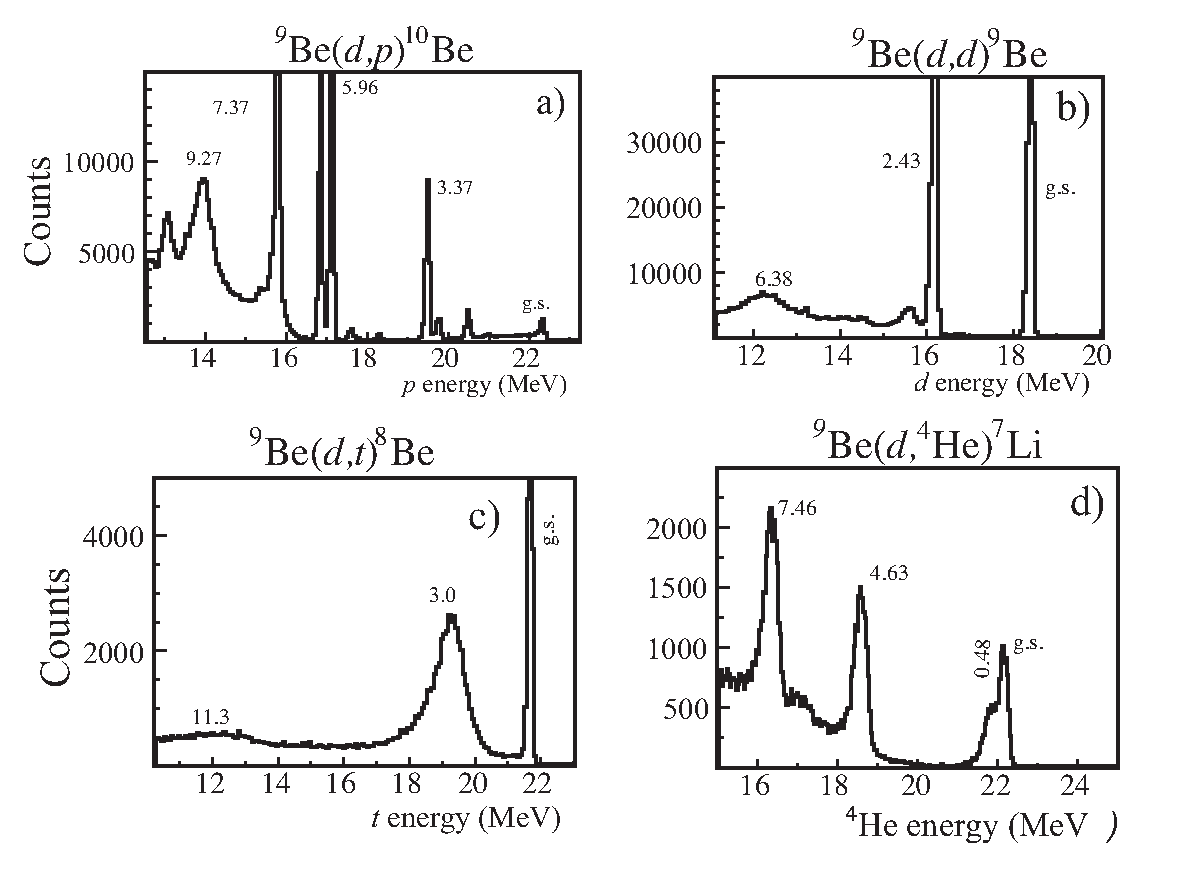
\includegraphics[width=8.2cm]{d_Etot_Fig2.eps}
\caption{Total deposited energy spectra measured at $\theta_{lab}$=32$^\circ$ for the detected $p$ (panel a), $d$ (panel b), $t$(panel c), and $\alpha$(panel d). The ground and the excited states of $^7$Li for the detected complementary product $\alpha$ as well as the ground states and the excited states for $^8$Be, $^9$Be, and $^{10}$Be in the case of detected $t, d$, and $p$, as complementary products, respectively, are unambiguously identified.}
\label{fig2}
\end{figure}	

%%%%%%%%%%%%%%%%%%%%%%%%%%%%%%%%
 The particles were identified based on the energy-loss measurements of $\Delta$E and the residual energy E$_r$, i.e., by the so-called $\Delta$E-E method. 
	An example of two-dimensional plots (yield vs. energy loss $\Delta$E and residual energy E$_r$) is shown in Fig.~\ref{fig1}.

The capability of current experimental technique is in identification of the particles $p, d, t$, and $\alpha$ and in the determination of their total deposited energies. The spectra of total deposited energy are shown in Fig.~2. All the peaks from Fig.~\ref{fig2} has been identified and assigned to the ground and the excited states of the $^{10}$Be, $^9$Be, $^8$Be, $^7$Li nuclei as the complementary products for the detected particles $p, d, t$, $\alpha$, respectively.





\section{Data Analysis and Results }
\subsection{Elastic scattering}


\begin{figure}[tp]
\centering
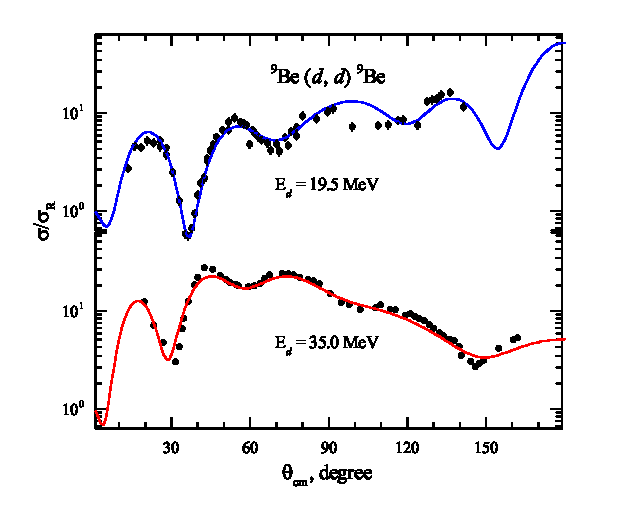
\includegraphics[width=8.2cm]{2H9BE.eps}
\caption{ \label{2H9BE}  \footnotesize The angular distributions of elastic scattering data of d from $^9$Be at laboratory energies 19.5~MeV (full circle) and 35~MeV (full triangle) in comparison with theoretical curves }
\end{figure}


\begin{table*}[bp]
\footnotesize
\caption{\label{potpar}  Potential parameters of the d+$^9$Be system used in the OM, the CC and the DWBA calculations.  }
\begin{tabular*}{\textwidth}{l l  @{\extracolsep{\fill}} l l l l l l l l l l   }
%\begin{tabular*}{\textwidth}{@{}cccccccccr@{\extracolsep{\fill}}c}
\br
E$_d$ &The  &	$V_0$, &	$r_V$, &	$a_V$, &	$W_D$, &	$r_D$, &	$a_D$, & $V_{SO}$, &	$r_C$	\\
MeV		& potential		& fm		&    fm		& MeV			& fm		& fm		& MeV			& fm			 \\
\mr
19.5 & DF	& \multicolumn{3}{c}{ $N_R=1.93^{ ~a)}$} &   14.89	&  0.63$^{ ~b)}$	&  0.854	& 5.56 &	0.809 	 \\
 ~& WS	& 57.32	 & 0.846	&  0.602 &  7.27	& 0.702	& 1.094 & $-$ & 0.809   \\
~ & CC 	& 77.87	 & 0.87	&  0.78 &  7.92	& 0.816	& 0.802 & 2.8 & 0.809   \\
35.0 &  DF	& \multicolumn{3}{c}{ $N_R=1.81^{ ~a)}$} &   14.27	& 0.63	&  0.88	& 5.56 &	0.809 	 \\
 ~& WS	& 64.03	 & 0.859	&  0.77 &  14.58	& 0.762	& 0.736 &$ -$ & 0.809   \\
 ~& CC 	& 73.9	 & 0.75	&  0.77 &  8.93	& 0.816	& 0.802 & 2.8 & 0.809  \\
%p + $^{10}$Be $^{b)}$ 		& 54.73 & 0.799 & 0.75 & 10.46 & 0.901 & 0.65 & 6.2 & 0.844 & $-$ & $-$  \\
%t + $^8$Be	$^{c)}$		& 147.67 & 0.607 & 0.722 & 12.7 $^{a)}$ & 0.715 & 1.157 & 3.88 & 0.826 & $-$ & $-$\\
%$\alpha$ + $^7$Li  $^{d)}$&  107.47 & 0.68  & 0.801 & 11.7 $^{a)}$ & 0.857 & 0.654 & $-$ & 0.71 & $-$ & $-$ \\
\br
\end{tabular*}
\scriptsize
$^{a)}$ The DF potential was taken as a real volume part of the optical potential with the $N_R$ parameter.  \\
$^{b)}$ Radii were taken as $r=\left( A^{\frac{1}{3}}_p+A^{\frac{1}{3}}_t \right)^{-1} R$.  \\
%$^{c)}$ Global optical parametrizations from [] at E$_t$= 14.9 MeV.  \\
%$^{d)}$ Global optical parametrizations from [] at E$_\alpha$= 12.33 MeV.  \\
\end{table*}

The theoretical calculations  of the deuteron  elastic scattering  on  $^9$Be have been made in the framework of the Optical Model (OM). Both 19.5 and 35 MeV  energies of the experimental data  were considered in the analysis.  The model suggests interaction between two colliding nuclei in the following way:

\begin{equation}\label{eqn:OP}
\begin{array}{l}
 U(R)=-V^{V}(R)-iW^{V}(R)+iW^D(R)+\\
~~~ ~~~~~~~+V^{SO}(R)( \mathbf{l} \cdot \mathbf{ \sigma } )+V^C(R),
\end{array}
 \end{equation}
where $V^{V}, W^{V}(R), W^D, V^{SO}, $ and $V^C$ are volume, imaginary volume and surface, spin-orbit and coulomb potentials, respectively. 
 In this work for real part of the optical potential  two types of the potential  were considered: the Double Folding potential (DF)
\begin{equation}
V^V(R) = N_R V^{DF}(R) 
\end{equation}
with normalization factor $N_R$ and the phenomenological potential as a Woods-Saxon (WS) potential:
\begin{eqnarray}
V^V(R) =  V^V_0 f^{R^V_0, a^V_0}(R), \\
 f^{R_0,a_0}(R)=\frac{1}{1+exp{\frac{R-R_0}{a_0}}}.
\end{eqnarray}

The DF potential was deduced based on the effective M3Y-Paris nucleon-nucleon potential and the densities of projectile and target nuclei. For instance, the density distribution of $^9$Be was undertaken within the framework of the three body model $\alpha+\alpha+n$ (see  \cite{urazbekov2016} for details).

The WS optical potential parameters were obtained by fitting the theoretical cross sections to the experimental data  at 19.5 MeV and 35 MeV energies. As a starting point, the global parametrizations were used from Ref. \cite{globalDeuteron}. 




\begin{figure}[tp]
\centering
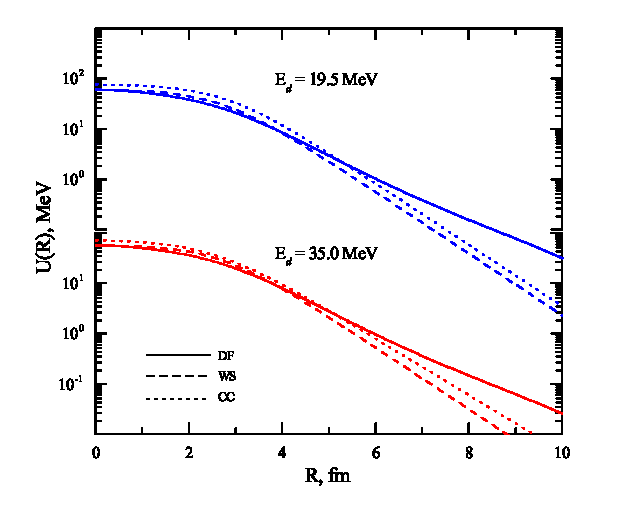
\includegraphics[width=8.2cm]{POT.eps}
\caption{ \label{POT}  \footnotesize Radial dependence of the optical potentials used in the elastic scattering analysis. }
\end{figure}



 The imaginary volume term is parametrized with the Wood-Saxon potential as well, while the surface and spin orbit terms have standard a form 
\begin{eqnarray}
W^D(R) &= -4 a_0^D W_0^D \frac{d}{dR} f^{R_0^D,a_0^D}(R), \\
V^{SO}(R) &= V_0^{SO}\left(\frac{\hbar}{m_\pi c}\right)^2 \frac{1}{R} \frac{d}{dR} f^{R_0^{SO} a_0^{SO}}(R).
\end{eqnarray}
The Coulomb term has been taken as the interaction of a point-charge with a uniformly charged sphere
\begin{eqnarray}
\label{coul}
V^C(R)= 
\cases{
\frac{Z_1 Z_2 e^2}{2 R_C} \left( 3- \frac{R^2}{R_C^2} \right) & for  R $\leq R_C$ \\
 \frac{Z_1 Z_2 e^2}{R} & for  R $> R_C$\\
 }
\end{eqnarray}

The values of elastic scattering in Fig.~\ref{2H9BE} are plotted in the scale of the ratio to Rutherford cross
section in comparison with the theoretical curves. Theoretical analyses were made within the optical model calculations using the DF potential (solid curve) and the WS potential (dashed curve).  Figure \ref{POT} shows the optical potentials used in the analysis of elastic scattering. The potential of double folding was as a real part of the optical potential, and its imaginary part was chosen empirically. 

A distinctive feature of the DF potential relative to empirical potentials is its slow convergence starting from $\sim 6$ fm. This is due to the matter density distribution of the neutron in $^9$Be, which also converges slowly (see \cite{urazbekov2016}). It also should  be noted that the potentials have almost identical behaviour in the region of the contact of colliding nuclei $\sim3.5-4.0$ fm. 
%The WS potential for 19 MeV has a fast convergence asymptotics caused to describe the front angles of scattering 20$^0$-30$^0$ with high accuracy. 
The potentials obtained in this way perfectly describe the elastic scattering cross section. The obtained potential parameters  are listed in Table \ref{potpar}.  


\begin{figure}[tp]
\centering
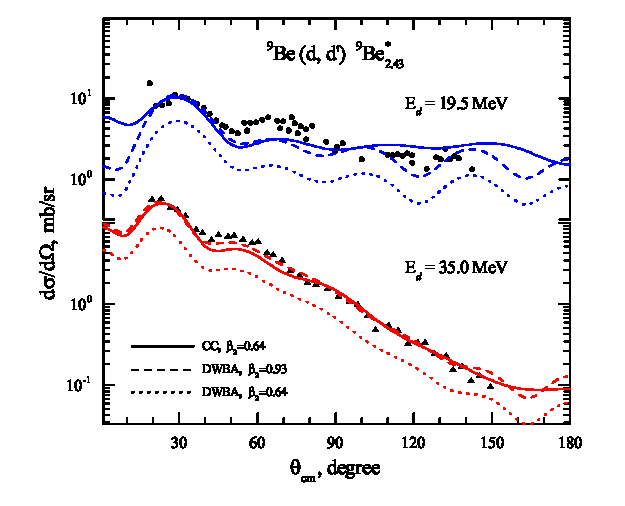
\includegraphics[width=8.2cm]{2H9BE2430MEV.eps}

\caption{\label{2H9BE2430MEV}The cross sections of inelastic scattering $^9$Be(d,d)$^9$Be* (E$_{exc}$=2.43 MeV) at laboratory energies 19.5 MeV (full circle) and 35 MeV (full triangle). Theoretical description explained in the text.}
\end{figure}

\subsection{Inelastic scattering}
The CC and the DWBA approaches have been applied to  analyse  inelastic scattering data with the target excitation of the  J$^{\pi}$=$\frac{5}{2}^-$ band. Calculations proceeded by means of the $FRESCO$ code \cite{fresco} and the $NRV$ project \cite{nrv}.

Spin reorientation effects of both the ground and excited states of $^9$Be  as well as  the band $\frac{7}{2}^-$ of $^9$Be were included into the coupling scheme.  It is suggested that the bands $\frac{5}{2}^-$ and $\frac{7}{2}^-$ mostly have a rotational nature. According to the CC approach, the interaction is modified taking into account the collective excitation by form factor:
%a correction taking into account target excitation to the interaction potential can be made by a form factor
\begin{equation}
V_\lambda(R)=-\frac{\beta_\lambda}{\sqrt{4\pi}} \frac{d U(R)}{dR},
\end{equation}
where $\beta_\lambda$ is the deformation parameter of  $\lambda$  multipole describing the target-nucleus form. 

The calculated cross sections for inelastic scattering are presented in Fig.~\ref{2H9BE2430MEV}. The theoretical analyses were made within the CC approach (solid curve) and within the DWBA approach (dashed and dot dashed curves) using  different values of the deformation parameter $\beta_2$. The potential used in the CC approach was taken in a such way that reproduces the cross section of inelastic scattering as well as elastic scattering data well (see Fig. \ref{2H9BE}). The parameters of the CC potential are listed in Table~\ref{potpar}.

The theoretical calculations made by means of the CC approach demonstrate good agreement with experimental data of angular distributions of inelastic scattering at energies 19.5 MeV and 35 MeV. The obtained quadrupole deformation parameter from the CC approach $\beta_2$ for the excited band $\frac{5}{2}^-$ reproduces data well and it is $\beta_2=0.64\pm0.03$, which corresponds to the previous studies \cite{lukyanov2014, harakeh1980}.

The DF potential was used  in the DWBA calculations for both the entrance channel and the exit channel. 
The DWBA calculations using the deformation parameter $\beta_2=0.64\pm0.03$ obtained by the CC calculations underestimate experimental data. However, it must be noted that in spite of the DWBA discrepancy the curve of this approach gives identical behaviour of the experimental data, which means the applicability of the DF potential. 

In order to get the best fit with the expermantal cross section of inelastic scattering in the framework of the DWBA approach, the deformation parameter must be increased up to $\beta_2=0.93\pm0.03$, or in the scale of deformation length up to $\beta R=0.93\cdot 1.25 A^{1/3}=2.418$ fm. Similar large values were also been reported in studies of Szczurek \etal  $ \beta R=3.7$ fm \cite{bodek1989},  Votava \etal  $\beta R=2.63$ fm \cite{votava1973} in the framework of the DWBA approach.

 
\begin{figure}[bp]
\centering
\includegraphics[scale=0.85]{9BE8BECC.eps}
\caption{ \label{9BE8BECC} The target coupling schemes in the $^9$Be(d,p)$^{10}$Be (upper) and the $^9$Be(d,t)$^8$Be (lower) nuclear reactions. The bold two headed arrows indicate E$\lambda$ transitions. The spin re-orientation effects are indicated as back pointing arrows.}
\end{figure}	

 It is well known the fact that taking into account the couplings of channels and the effects of spin re-orientation enhances the cross section. It leads to the reduction of the value of the deformation parameter. However, the DWBA approach is not able to cover these effects. Therefore, the value of the deformation parameter must be increased  in order to compensate the difference of the DWBA cross sections with experiment. 

%The implementation of the CC approach is demonstrating a good agreement with angular distributions of inelastic scattering data. Exact matching value of the deformation parameter with other theoretical researches has been obtained. Generally it can be concluded that  strong coupling effects between channels exist in $^9$Be(d,d)$^9$Be$^*$.
%In accordance with a good agreement of experimental data with both theoretical angular distributions and obtained deformation parameter within the CC approach it should therefore be noted that there exist strong coupling effects between channels.



 




\subsection{One nucleon transfer reactions } 
Rearrangement nuclear reactions with one nucleon have been analyzed within the framework of both the Coupled Reaction Channels (CRC) and the DWBA approaches. 
 
\begin{figure}[tp]
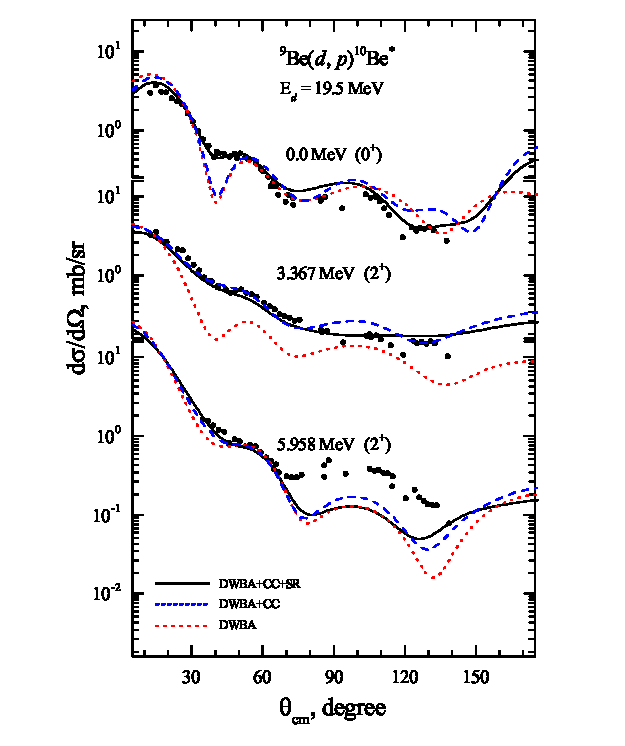
\includegraphics[scale=0.8]{1H10BE.eps}
\caption{\label{1H10BE} Differential cross sections for the ground and low-lying excited states of $^{10}$Be  produced in the d + $^9$Be nuclear reaction at 19.5 MeV. Experimental data are in comparison with  theoretical curves obtained with the CRC and the DWBA methods.  }
\end{figure}

\begin{figure}[tp]
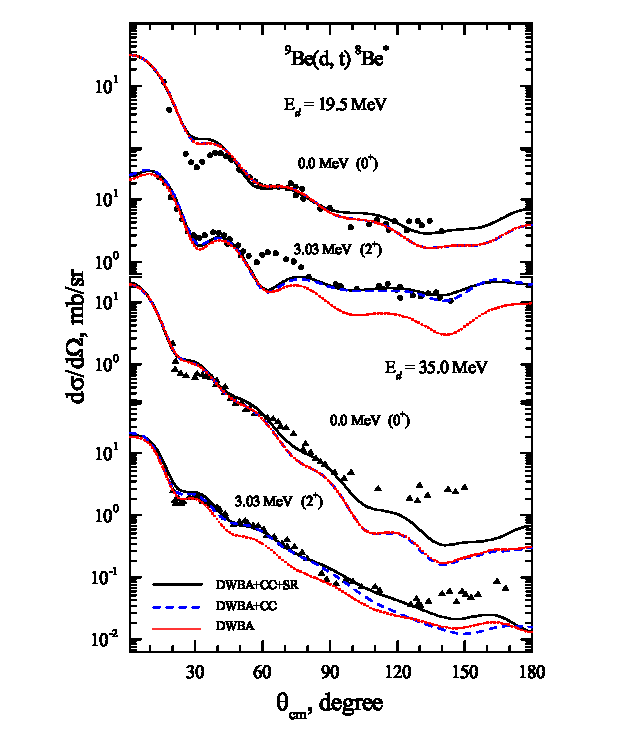
\includegraphics[scale=0.8]{3H8BE.eps}
\caption{
\label{3H8BE} 
Differential cross sections of the ground and low-lying excited states of $^{8}$Be produced in the d + $^9$Be reaction at both 19 MeV and 35 MeV energies. The experimental data are shown in comparison with  theoretical curves calculated within the CRC and the DWBA methods.}
\end{figure}

The DF potential was assigned as a potential for the entrance channel for DWBA calculations, and the global optical parametrizations for the exit channels were used from Ref. \cite{globalProton, globalTriton}.  The DWBA transition amplitude in the framework of this approach has been taken in prior form for both reactions. Wave functions of relative motion between the transferred particle and the core have been built on the Woods-Saxon potential with a depth fitted to the bound energy, radius $R=1.25 A_{com}^{1/3}$ and diffuseness $a=0.65$. The depth of the potential was applied 0.1 MeV in exceptional cases when the valence was not bound, as it was suggested in Ref. \cite{harakeh1980}. If the core and the composite nuclei have internal excitation energies, a renewed binding energy $BE^{\star}$ of the transferred particle is expressed by the formula:
\begin{equation}
BE^{\star}=BE - E_{com}^*+E_{core}^*
\end{equation}
where $BE$ $-$ the binding energy of the transferred particle, $E_{com}^*,~E_{core}^*~-$  excitation energies of the composite and  core nuclei, respectively.

The spectroscopic amplitudes for one particle states were calculated by means of the $ANTOINE$ code \cite{antoine}  using the effective Cohen-Kurath interaction for $p$-shell nuclei \cite{cohen1965}. In particular, the spectroscopic amplitude  $S$ for an addition of nucleon from a specific initial state $J'$ to a specific final state $J$ is related to the matrix element of the creation operator $\hat{a}^\dagger$ or the destruction operator $\hat{a}$ \cite{brown2017}:
\begin{equation}
\label{eq:SA}
\begin{array}{l}
S=\frac{\langle J~ k^n \Vert \hat{a}^\dagger \Vert J' ~k^{n-1} \rangle}{\sqrt{2J+1}} \\
~~=(-1)^{j+J-J'} \frac{\langle J'~ k^{n-1} \Vert \hat{a} \Vert ~ J ~k ~\rangle}{\sqrt{2J+1}}.
\end{array}
\end{equation}
where $k$ stands for the set of single-particle quantum numbers $nlj$.  The calculated spectroscopic amplitudes for the one nucleon transfer reactions are listed in Tab.\ref{SA}.


\begin{table*}[tp]
\footnotesize
\caption{\label{SA}  Spectroscopic amplitudes used in CRC calculations for the Composite = Core + Cluster system. The one nucleon Spectroscopic Amplitudes calculated by means of the $ANTOINE$ code \cite{antoine}. The alpha spectroscopic amplitudes were taken from  \cite{volya, volya2017}. }
\begin{tabular*}{\textwidth}{@{\extracolsep{\fill}}llllllrl@{\extracolsep{\fill}}llllllr@{\extracolsep{\fill}}}
\br
Composite & 2J$_{com}$ & Core & 2J$_{core}$ & Cluster & 2J & SA &    & Composite & 2J$_{com}$ & Core & 2J$_{core}$ & Cluster & 2J & SA      \\
\mr
$^9$Be  & 3  & $^8$Be   & 0   & n       & 3   & -0.761 &  & $^9$Be  & 3  & $^8$Li   & 2$_1$    & p       & 1   & -0.444  \\
$^9$Be  & 3  & $^8$Be   & 4   & n       & 3   & 0.816  &  & $^9$Be  & 3  & $^8$Li    & 6   & p       & 3   & -0.592  \\
$^9$Be  & 3  & $^8$Be   & 4   & n       & 1   & -0.242 &  & $^9$Be  & 3  & $^8$Li    & 2$_2$   & p       & 3   & -0.236  \\
$^9$Be  & 5  & $^8$Be   & 4   & n       & 3   & 0.986  &  & $^9$Be  & 3  & $^8$Li    & 2$_2$   & p       & 1   & 0.036   \\
$^9$Be  & 5  & $^8$Be   & 4   & n       & 1   & -0.417 &  & $^9$Be  & 5  & $^8$Li    & 4   & p       & 3   & 0.593   \\
$^9$Be  & 5  & $^8$Be   & 8   & n       & 3   & -0.374 &  & $^9$Be  & 5  & $^8$Li    & 4   & p       & 1   & 0.515   \\
$^9$Be  & 7  & $^8$Be   & 4   & n       & 3   & -0.457 &  & $^9$Be  & 5  & $^8$Li   & 2$_1$    & p       & 3   & -0.672  \\
$^9$Be  & 7  & $^8$Be   & 8   & n       & 3   & 0.919  &  & $^9$Be  & 5  & $^8$Li    & 6   & p       & 3   & -0.571  \\
$^9$Be  & 7  & $^8$Be   & 8   & n       & 1   & -0.429 &  & $^9$Be  & 5  & $^8$Li    & 6   & p       & 1   & -0.171  \\
$^8$Be  & 0  & $^7$Li   & 3   & p       & 3   & -1.204 &  & $^9$Be  & 5  & $^8$Li    & 2$_2$   & p       & 3   & 0.2     \\
$^8$Be  & 0  & $^7$Li   & 1   & p       & 1   & 0.736  &  & $^9$Be  & 7  & $^8$Li    & 4   & p       & 3   & -0.323  \\
$^8$Be  & 4  & $^7$Li   & 3   & p       & 3   & -0.748 &  & $^9$Be  & 7  & $^8$Li    & 6   & p       & 3   & -0.899  \\
$^8$Be  & 4  & $^7$Li   & 3   & p       & 1   & -0.612 &  & $^9$Be  & 7  & $^8$Li    & 6   & p       & 1   & -0.564  \\
$^8$Be  & 4  & $^7$Li   & 1   & p       & 3   & 0.667  &  & $^7$Li  & 3  & $^6$Li   & 2   & n       & 3   & 0.657   \\
$^8$Be  & 4  & $^7$Li   & 7   & p       & 3   & 0.624  &  & $^7$Li  & 3  & $^6$Li   & 2   & n       & 1   & -0.538  \\
$^8$Be  & 4  & $^7$Li   & 5$_2$   & p       & 3   & 0.079  &  & $^7$Li  & 3  & $^6$Li   & 6   & n       & 3   & 0.744   \\
$^8$Be  & 4  & $^7$Li   & 5$_2$   & p       & 3   & -0.146 &  & $^7$Li  & 3  & $^6$Li   & 4   & n       & 3   & -0.032  \\
$^8$Be  & 8  & $^7$Li   & 7   & p       & 3   & 0.864  &  & $^7$Li  & 3  & $^6$Li   & 4   & n       & 1   & 0.399   \\
$^8$Be  & 8  & $^7$Li   & 7   & p       & 1   & 0.687  &  & $^7$Li  & 1  & $^6$Li   & 2   & n       & 3   & -0.925  \\
$^8$Be  & 8  & $^7$Li   & 5$_2$   & p       & 3   & 0.374  &  & $^7$Li  & 1  & $^6$Li   & 2   & n       & 1   & 0.197   \\
$^8$Li  & 4  & $^7$Li   & 3   & n       & 3   & -0.988 &  & $^7$Li  & 1  & $^6$Li   & 4   & n       & 3   & -0.555  \\
$^8$Li  & 4  & $^7$Li   & 3   & n       & 1   & 0.237  &  & $^7$Li  & 7  & $^6$Li   & 6   & n       & 3   & -0.936  \\
$^8$Li  & 4  & $^7$Li   & 1   & n       & 3   & 0.43   &  & $^7$Li  & 7  & $^6$Li   & 6   & n       & 1   & 0.645   \\
$^8$Li  & 4  & $^7$Li   & 7   & n       & 3   & -0.496 &  & $^7$Li  & 7  & $^6$Li   & 4   & n       & 3   & -0.456  \\
$^8$Li  & 4  & $^7$Li   & 5   & n       & 3   & -0.665 &  & $^7$Li  & 5$_2$  & $^6$Li   & 2   & n       & 3   & -0.650   \\
$^8$Li  & 4  & $^7$Li   & 5$_2$   & n       & 1   & -0.275 &  & $^7$Li  & 5$_2$  & $^6$Li   & 6   & n       & 3   & 0.732   \\
$^8$Li  & 2$_1$  & $^7$Li   & 3   & n       & 3   & 0.567  &  & $^7$Li  & 5$_2$  & $^6$Li   & 6   & n       & 1   & 0.549   \\
$^8$Li  & 2$_1$  & $^7$Li   & 3   & n       & 1   & 0.351  &  & $^7$Li  & 5$_2$  & $^6$Li   & 4   & n       & 3   & 0.200     \\
$^8$Li  & 2$_1$  & $^7$Li   & 1   & n       & 3   & 0.905  &  & $^7$Li  & 5$_2$  & $^6$Li   & 4   & n       & 1   & -0.114  \\
$^8$Li  & 2$_1$  & $^7$Li   & 1   & n       & 1   & 0.331  &  & $^6$Li  & 2  & d     & 2   & $\alpha$     & 0   & 0.907  \\
$^8$Li  & 2$_1$  & $^7$Li   & 5$_2$   & n       & 3   & 0.767  &  & $^6$Li  & 2  & d     & 2   & $\alpha$     & 4   & 0.077   \\
$^8$Li  & 6  & $^7$Li   & 3   & n       & 3   & 0.581  &  & $^6$Li  & 6  & d     & 2   & $\alpha$     & 4   & 0.943   \\
$^8$Li  & 6  & $^7$Li   & 5$_2$   & n       & 3   & -0.66  &  & $^6$Li  & 6  & d     & 2   & $\alpha$     & 8   & 0.028   \\
$^8$Li  & 6  & $^7$Li   & 5$_2$   & n       & 1   & -0.541 &  & $^6$Li  & 4  & d     & 2   & $\alpha$     & 4   & 0.929   \\
$^8$Li  & 6  & $^7$Li   & 7   & n       & 3   & 0.973  &  & $^9$Be  & 3  & $^5$He   & 3   & $\alpha$     & 0   & -0.925  \\
$^8$Li  & 6  & $^7$Li   & 7   & n       & 1   & -0.404 &  & $^9$Be  & 3  & $^5$He   & 3   & $\alpha$     & 4   & 0.784   \\
$^8$Li  & 2$_2$  & $^7$Li   & 3   & n       & 3   & -0.617 &  & $^9$Be  & 5  & $^5$He   & 3   & $\alpha$     & 4   & 0.974   \\
$^8$Li  & 2$_2$  & $^7$Li   & 3   & n       & 1   & -0.841 &  & $^9$Be  & 5  & $^5$He   & 3   & $\alpha$     & 8   & -0.26   \\
$^8$Li  & 2$_2$  & $^7$Li   & 1   & n       & 3   & 0.178  &  & $^9$Be  & 7  & $^5$He   & 3   & $\alpha$     & 4   & 0.882   \\
$^8$Li  & 2$_2$  & $^7$Li   & 1   & n       & 1   & 0.331  &  & $^9$Be  & 7  & $^5$He   & 3   & $\alpha$     & 8   & -0.737  \\
$^8$Li  & 2$_2$  & $^7$Li   & 5   & n       & 3   & 0.231  &  & $^7$Li  & 3  & t     & 1   & $\alpha$     & 1   & 0.970       \\
$^9$Be  & 3  & $^8$Li    & 4   & p       & 3   & -0.947 &  & $^7$Li  & 1  & t     & 1   & $\alpha$     & 1   & 0.961       \\
$^9$Be  & 3  & $^8$Li    & 4   & p       & 1   & -0.319 &  & $^7$Li  & 7  & t     & 1   & $\alpha$     & 3   & 0.952       \\
$^9$Be  & 3  & $^8$Li    & 2$_1$   & p       & 3   & 0.454  &  & $^7$Li  & 5$_2$  & t     & 1   & $\alpha$     & 3   & 0.223  \\
\br
\end{tabular*}
\end{table*}



\begin{figure*}[bp]
\centering
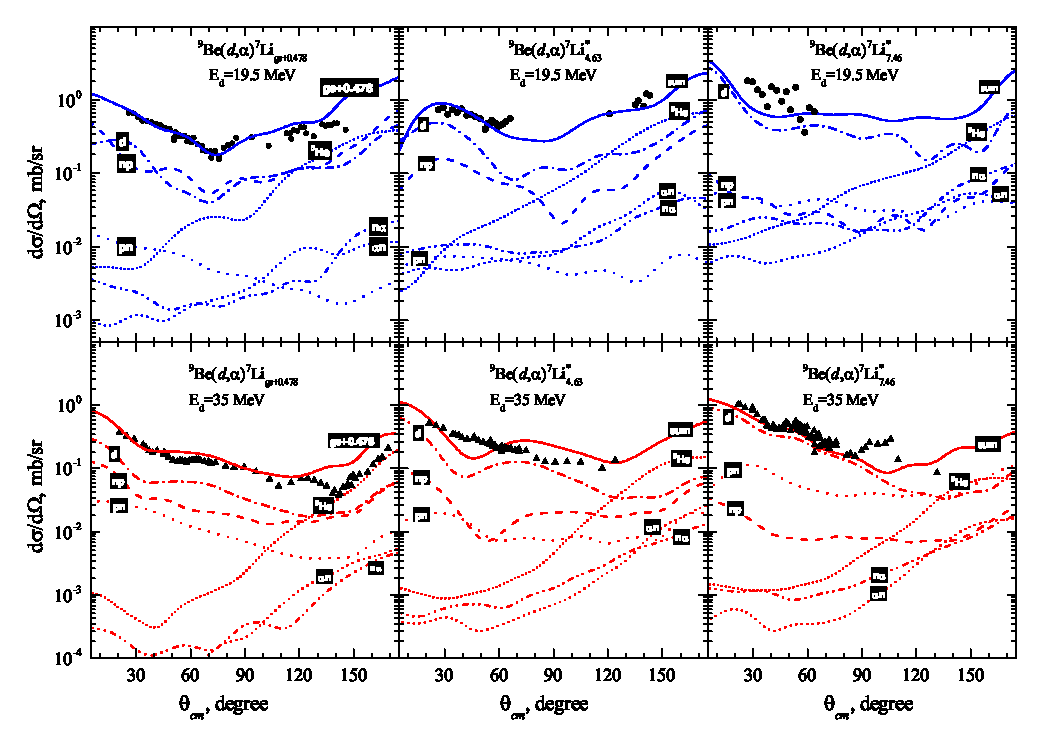
\includegraphics[scale=0.9]{4HE7LI.eps}
\caption{\label{label} Differential cross sections for the ground and low-lying excited states of $^{7}$Li  produced in the d + $^9$Be reaction at  both 19.5 MeV and 35 MeV. }
\label{4HE7LI}
\end{figure*}	 

The CC potentials were used in the CRC calculations for the entrance channel. The coupling schemes of target nuclei for the $^9$Be(d,p)$^{10}$Be and $^9$Be(d,t)$^8$Be  reactions  are illustrated in Fig. \ref{9BE8BECC}. The states of $^{10}$Be,   $2^+_{1}$ and $2^+_{2}$, as well as the low-lying excited states of $^8$Be,  $2^+$ and $4^+$, were implemented to the coupling scheme. Also, the schemes take into account the spin reorientation effects of states on the condition $J\neq0$. 


Angular distributions of the $^9$Be(d,p)$^{10}$Be and  $^9$Be(d,t)$^{8}$Be nuclear reactions are shown in the Fig. \ref{1H10BE} and \ref{3H8BE}, respectively. Theoretical calculations with the use of CRC approach  are in excellent agreement with experimental data. The analysis shows  the importance of taking into account the channel coupling and spin reorientation effects, if one excludes the direct DWBA transitions: $^9$Be$^{gs}\rightarrow^8$Be$^*$ and $^9$Be$^{gs}\rightarrow^{10}$Be$^*$. The contribution of these components are indicated as CC+SR in Fig. \ref{1H10BE}-\ref{3H8BE}.


The investigation of two-step transfer mechanism of the $^9$Be(d,p)$^{10}$Be nuclear reaction at E$_d$=15 MeV was conducted in Ref. \cite{galanina2012}. The study revealed a dominant contribution of the two step process, i.e. neutron pickup and dineutron stripping, at the forward scattering angles. Compared to this theoretical description, our approach to the analysis of the $^9$Be(d,p)$^{10}$Be nuclear reaction provides better agreement with the experimental data. 

The applicability of the CRC approach to  the $^9$Be(d,p)$^{10}$Be and $^9$Be(d,t)$^{8}$Be nuclear reactions, including the excited states and spin reorientations, points to the fact that there are strong coupling channel effects in both entrance and exit channels. This kind  of effects was also enhanced in Ref. \cite{harakeh1980, rudchik2016}. 


\begin{figure}[tp]
\centering
\includegraphics[scale=0.8]{4HE7LiCC.eps}
\caption{\label{4He7LICC} The scheme illustrating mechanisms in the $^9$Be(d,$\alpha$)$^7$Li reaction for the CRC calculations. }
\end{figure}	


\subsection{Cluster transfer reaction}
Differential cross sections for the nuclear reaction  ${^9}$Be($d$,$\alpha$)$^7$Li are of particular interest. The reason is in abnormality at large scattering angle. This fact gives a suggestion of heavy cluster transfer $^5$He. Moreover, the cross section calculated within the DWBA approach gives underestimated values even at forward angles of scattering. Therefore, in order to cure the distinction between theory and experiment, the following transfer mechanisms are suggested (see Fig. \ref{4He7LICC}): 
\begin{itemize}
\item[$-$] direct transfer: $d$, $^5$He ;
\item[$-$] sequential transfer of systems: n-p, p-n, n-$\alpha$ and $\alpha$-n;
\end{itemize}

The transition amplitudes of transferring  the heavy cluster $^5$He, the n-$\alpha$ system and the $\alpha$-n system have been inverted depending on the scattering angles:
\begin{equation}
\label{eq:ampl1}
f_{I}(\theta)=f_{^5He}(\pi - \theta) + f_{n-\alpha}(\pi - \theta) + f_{\alpha-n}(\pi - \theta) 
\end{equation}
while the amplitudes of transferring  d, the n-p  and  p-n systems is
\begin{equation}
\label{eq:ampl2}
f_{II}(\theta)=f_{d}(\theta) + f_{n-p}( \theta) + f_{p-n}(\theta) 
\end{equation} 
The resulting differential cross section for the nuclear reaction ${^9}$Be($d$,$\alpha$)$^7$Li is given by a coherent sum of amplitudes from Eq.\ref{eq:ampl1} and Eq.\ref{eq:ampl2}
\begin{equation}
\frac{d\sigma}{d\Omega}=\vert f_{I}(\theta) + f_{II}(\theta) \vert ^2.
\end{equation}

The quantum numbers of transferred clusters $NL_J$ have been constructed by conservation of the total number of oscillation quanta $\mathcal{N}$ \cite{satchler1983}
\begin{equation}
\mathcal{N} =2(N-1)+L=\sum_{i} \left( 2 \left( n_i -1 \right) + l_i \right),
\end{equation}
where $i -$ the number of each constituent nucleon in the cluster, $n_i l_i -$ the quantum numbers of $i$-indexed nucleon,
and by the triangle law of inequality:
\begin{equation}
\vert {J}_{com} - {J}_{core} \vert \le {J} \le \vert {J}_{com} + {J}_{core} \vert,
\end{equation}
where $J_{com}$, $J_{core}$ are the spin numbers of composite and core nuclei, respectively. 

 The CC potential (see Tab.~\ref{potpar}) for the entrance channel and global optical potentail parametrizations from Ref. \cite{globalTriton, globalAlpha, global6Li} for intermediate and exit channels have been used in analysis. For two-step transfer reactions, the transition amplitudes were calculated in the prior form for the first coupling, then in the post form for the second coupling. The spectroscopic amplitudes for d and $^5$He were taken from Ref. \cite{fiveSA}; for one nucleon and alpha transfer transitions are shown in Tab.~\ref{SA}.
 
 
Figure \ref{4HE7LI} shows the results of calculations of the angular distributions  for the $^9$Be(d,$\alpha$)$^7$Li nuclear reaction with low-lying excited states of the $^7$Li nucleus. The cross sections are calculated for energies at 19 MeV (upper part) and 35 MeV (lower part). In fig.\ref{4HE7LI}  it can be seen that in all the channels the transfer of the deuteron  has mainly the dominant contribution. Despite the fact that the spectroscopic amplitude of the deuteron 0.558 with quantum numbers ${1\textrm{D}_3}$ \cite{bodek1989} in the $^9$Be nucleus is not of great importance, a noticeable cross section is due to the large value of the deuteron spectroscopic amplitude  1.732 with the configuration ${1\textrm{S}_1}$ in $^4$He. It should be noted that the contribution of the deuteron transfer mechanism to the cross section mainly occurs with the wave ${1\textrm{D}_3}$ in the background with other waves, such as ${2\textrm{S}_1}, 1\textrm{D}_1, 1\textrm{D}_2$. It is important to note that the behaviour of the ${1\textrm{D}_3}$ wave converges very slowly with respect to the angle, which is almost identical to the angular distribution of evaporation residues.

In all channels starting from angle 120, the transfer of the $^5$He cluster has a predominant contribution.
It is interesting to note that the transfer of the $^5$He cluster  basically occurs simultaneously in exit channels with all excited states of $^7$Li. The first such results were obtained in Ref. \cite{bodek1989} . In this paper, an analysis of the nuclear reaction with a laboratory energy of 7 MeV was carried out with the assumption that the $^5$He cluster  is transferred simultaneously, neglecting the sequential transfer. Using the CRC method, we could estimate the contribution of the sequential transfer of the $^5$He cluster, which is not represented anywhere. It turned out that the n-$\alpha$ and the $\alpha$-n transfer processes really had a smaller contribution by an order of magnitude lower than the simultaneous transfer. Simultaneous transfer of the $^5$He cluster was also represented as a dominant process than the sequential one by Jarczyk \etal \cite{jarczyk1996} on the example of the $^{12}$C($^{11}$B, $^6$Li)$^{17}$O and $^{12}$C(d, $^7$Li)$^{7}$Be nuclear reactions. Nevertheless, it should be noted that  the n-$\alpha$ and the $\alpha$-n transfer processes are beginning to have a significant contribution as the excitation energy of $^7$Li increases, where they should not be ignored.

The next mechanism, which has a rather noticeable contribution to the cross section, is the transfer of the n-p system. A significant contribution is due to the cluster structure of the $^9$Be nucleus, i.e. the weakly bound neutron. The results of calculations show that the contribution of transfer of  the p-n system is much lower than the contribution of the n-p system. It is interesting to note that similar results were obtained in Ref. \cite{coker1974}. In this paper, the treatment of the DWBA discrepancy in the $^{98}$Mo(d,$\alpha$)$^{96}$Nb direct deuteron transfer reaction was gained by coherently adding the two-step processes. In particular, the calculations have shown that the (d,t;t,$\alpha$) process prevails over the (d,$^3$He;$^3$He,$\alpha$) process.

 Figure \ref{CS} shows the results of calculations of the integrated cross sections for each mechanism in the $^9$Be(d,$\alpha$)$^7$Li nuclear reaction. The contribution to the cross section can be made in the following order: direct transfer of the deuteron, transfer of the n-p system, transfer of a heavy $^5$He cluster,  and sequential  transfer of the p-n, a-n, and n-a systems. However, the order of the contribution of the p-n and $^5$He mechanisms changes when the laboratory energy reaches a value of 100 MeV.
%The results of calculations show that the more excitation energy of the $^7$Li nucleus, the less contribution of the n-p system is given, the more contribution of the p-n system. 
 
 
 
 
 


\begin{figure}[tp]
\centering
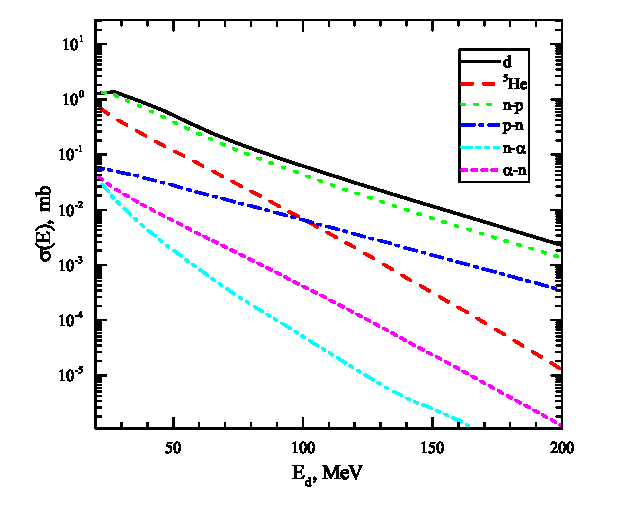
\includegraphics[width=8.2cm]{CS.eps}
\caption{\label{CS} Integrated cross sections depending on laboratory energy E$_d$ for each mechanism: d, $^5$He, n-p, p-n, n-$\alpha$ and $\alpha$-n. }
\end{figure}	
	
\section{Conclusion}
In the present work, the nuclear reactions induced by interaction of deuteron with $^9$Be  have been analysed. The following conclusions can be made during the analysis:
\begin{itemize}
\item The double-folding potential, which is characteristic of the interaction of deuteron with $^9$Be, differs from phenomenological optical potentials;
\item  The deformation parameter has been obtained for the excited state 2.43 MeV of $^9$Be;
\item The strong coupling effects in the nuclear reactions with one nucleon transfer have been revealed;
\item It was found that  in the $^9$Be(d,$\alpha$)$^7$Li nuclear reaction the $^5$He heavy cluster  is transferred mainly simultaneously, and the contribution of its sequential transfer is an order of magnitude lower;
\item The importance of taking into account the mechanism of sequential transfer of the n-p system has been revealed.
\end{itemize}

\ack
	The authors acknowledge the support of the CANAM project \cite{canam} for providing beam time for the experiment. The authors also grateful to I. Thompson for advising on FRESCO code and to A. Volya for giving the alpha spectroscopic amplitudes. 
	
	This work was supported by the Russian Science Foundation (17-12-01170) and by the Program of the Ministry of Education and Science of Kazakhstan (IRN~AP05132978) 



\section*{References}

\bibliographystyle{iopart-num}
%\begin{thebibliography}
\bibliography{urazbekov}
%\end{thebibliography}







\end{document}

